\documentclass[10pt,a4paper]{article}
\usepackage[utf8x]{inputenc}
\usepackage[french]{babel}
\usepackage[T1]{fontenc}
\usepackage{amsmath}
\usepackage{amsfonts}
\usepackage{amssymb}
\usepackage{graphicx}
\usepackage{verbatim}
\author{Paul Fayoux}
\title{Algorithme de recherche de stable}
\begin{document}

\section{Algorithme}

\paragraph{Algorithme de base}

\begin{verbatim}
Structure globale :
T, l’ensemble des ensembles stables maximum
taille, la taille d’un ensemble stable maximum
Entrée:
Un graphe non orienté G= [S,A].
Un ensemble stable en cours de calcul Ss
Sortie: Rien
1: function EnuStableMax(G,Ss)
2: Si (S=Æ) Alors
3: Si (|Ss|>taille) Alors
4: Vider T et taille ← 0
5: T ← {Ss} et taille ← |Ss|
6: Sinon Si (|Ss|=taille) Alors
7: T ← {Ss}
8: FinSi
9: FinSi
10 : Sinon
11: Pour i=1 à |S| Faire
12: s ← S[i] // s est le sommet en position i dans la liste des sommets restants S
13: Ss ← Ss+ {s}
14: S ← S - {s}
15: Retirer de S tous les sommets ayant une arrête commune avec s
16: EnuStableMax(G,Ss)
17: Remettre dans S les sommets supprimés à l’étape 14 et 15
18: Fin Pour
19: Fin Si
\end{verbatim}

Cette fonction parcours l'ensemble des sommets du graphe, puis prélève un premier sommet du graphe l'ajoute à la solution puis supprime les sommets liés à ce sommet prélevé et recommence l'opération jusqu'à ce qu'il n'y ai plus de sommet à parcourir. On calcule ainsi l'ensemble des stables possible du graphe et on ne garde que ceux qui ont la taille la plus grande.
\\
Cet algorithme est facilement réalisable, mais il n'est pas très efficace.

\paragraph{Voici plusieurs point qu'il semble intéressant de chercher à améliorer :}

\begin{itemize}
\item On s'aperçoit dans un premier temps que chaque stable calculé au cours de l'algorithme est recalculé autant de fois qu'il y a de sommet dans ce stable, l'algorithme ne détecte pas si il a déjà trouvé un stable et considère deux stables différents si ils ont un ordre de sommet différent. \\ 
Il serait donc intéressant de pouvoir limité ces calculs inutiles.
\\\\
\item Si on s'intéresse au pire des cas pour notre algorithme, on s'aperçoit que moins le graphe ne comporte d'arête, moins les sommets sont liés et plus l'algorithme sera long. Dans notre algorithme le pire des cas et un graphe sans arête où tous les sommets sont déjà indépendants (on obtient un temps maximum de $n!$ avec $n$ le nombre de sommets).
\\\\
\item Lorsque notre algorithme tourne, les sommets sont pris " au hasard " dans l'ordre dans lequel ils ont été numéroté. Si on choisie de prendre les sommets arbitrairement selon une certaine règle on peut peut-être amélioré l'algorithme.
\end{itemize}

\paragraph{Voici les améliorations qui pourraient être faites : }

\begin{itemize}
\item Dans le cas des solutions recalculées, il ne semble pas évident de pouvoir vérifier qu'une solution ai été déjà calculé, nous verrons plus tard si une amélioration peut-être réalisable.
\\
\item Par contre, en ce qui concerne le pire des cas, on sait déjà que l'on peut créé une règle permettant d'ajouter automatiquement tout les sommets du graphes qui n'ont aucune arêtes dans la solution (car ils y seront nécessairement). Mais une fois cette règle mise en place, le pire des cas revient à un graphe qui aurait n paires de sommet reliés par une arête, en imaginant que l'on fasse une autre règle spécifique pour ce cas précis, on ne ferait que décaler le problème à un graphe qui aurait $n$ ensemble de sommet reliés entre eux. Ce qui nous amène à considérer ce problème de façon plus large, en réalité ce qui se cache derrière tout ceci est de savoir si notre graphe est connexe ou non. Dans le cas ou le graphe n'est pas connexe, on peut savoir que si $n$ est le nombre de parties connexe qui forment le graphe, le nombre minimum de sommets dans un stable est $n$. Si on arrive à diviser le graphe non connexe en plusieurs graphe connexe il ne reste alors qu'à faire tourner l'algorithme sur chacun de ces sous graphe et on aurait la solution optimale du stable maximum.
\\
Si l'on s'intéresse à la connexité d'un graphe, on peut même aller plus loin. Si l'on considère un graphe  connexe, on peut le diviser en plusieurs ensembles connexes, puis chercher le stable maximum pour chacun de ses sous graphes et rassembler les résultats pour obtenir notre solution. Cette amélioration diminue grandement la complexité de notre algorithme en limitant le pire des cas (il reste à déterminer un moyen de faire cela). Si l'on prend un graphe qui se divise en deux sous graphes connexes reliés entre eux par une arête (figure 1) , il parait évident que l'on peut diviser ce graphe en deux sous graphes puis recalculer les solutions en enlevant l'un ou l'autre des sommets qui servent à la liaison des deux graphes (si ils apparaissent dans les sous solutions).
\\

\item Concernant le choix des sommets lors du parcours, on peut déjà avant même de travailler sur le graphe ordonner ses sommets par ordre croissant de nombre d'arêtes avec un tri rapide. Cela permet de parcourir en priorité les sommets qui ont un faible nombre d'arête, ce qui normalement permet d'obtenir une solution optimale plus rapidement. Cela revient à choisir le sommet ayant le nombre d'arête minimum à chaque fois dans l'ensemble des sommets restant. On pourrait aussi rajouter une règle faisant arrêter l'algorithme dès lors que l'on part d'un sommet ayant un nombre d'arêtes trop grand pour que l'on puisse tomber sur une solution qui soit optimale.\\\\
\end{itemize}

\textit{Remarque :} Lorsque l'on regarde l'ensemble des stables maximums pour un graphe donné, on s'aperçoit qu'un ensemble de sommets apparait à chaque fois dans ces solutions seuls certains sommets changent. Y a-il un moyen permettant de connaitre cette ensemble afin de trouver les solutions plus rapidement ?

\begin{figure}[h]
 \hspace{-4cm}
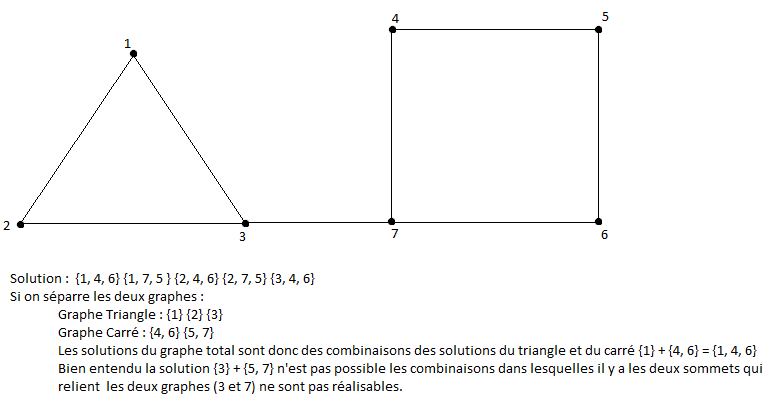
\includegraphics[scale=1]{image1.png}
\end{figure} 

Ils nous reste à déterminer un algorithme afin de diviser un graphe en sous graphe connexe.

Il existe deux notions liés à la connexité dans les graphes non orienté, à savoir les points d'articulation et les isthmes. Un point d'articulation est un sommet qui augmente le nombre de connexité si on l'enlève, un isthme est une arête ayant la même propriété. Ces deux notions pourraient nous permettre de divisé un graphe en sous partie connexe (on obtiendrait un graphe $k$-connexe).

En cherchant rapidement, on trouve facilement un algorithme pour la recherche de point d'articulation celui-ci aurait une complexité en $O(nm)$ avec $n$ le nombre de sommet et $m$ le nombre d'arêtes. 

La notion de communauté est aussi intéressante, une communauté étant un ensemble de nœuds ayant de nombreuse connexions entre eux mais ayant un très faible nombre de connexion vers l'extérieur.

L'algorithme de Girvan-Newman permet de déterminer des communautés dans un graphe, sa complexité est assez forte $O(n^3)$ cependant cette complexité reste moindre par rapport à celle de notre algorithme (elle est en temps polynomial , notre algorithme ne l'est pas). Cela veut dire qu'il serait intéressant d'appliquer cet algorithme si on travaille sur des grandes instances.

\section{Avancement dans le projet}

Afin de pouvoir de pouvoir tester nos algorithme nous avons créé un graphe de test :

\begin{figure}[h]
 \hspace{-4cm}
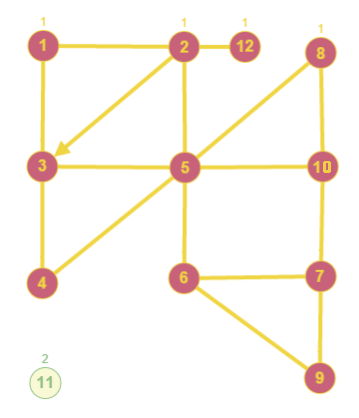
\includegraphics[scale=1]{exemplegraphe.png}
\end{figure} 

Nous avons pu alors tester notre algorithme de base afin d'obtenir les solutions suivantes :

\begin{enumerate}
\item ${1, 4, 8, 9, 11, 12}$
\item ${1, 4, 6, 8, 11, 12 }$
\item ${1, 4, 7, 8, 11, 12 }$
\end{enumerate}

Nous avons créé un algorithme plus rapide choisissant en priorité les sommets ayant le moins de d'arête.

\subsection{Rapport 12/10/2015}

Durant la semaine, nous avons corrigé un certain nombre de bugs liés à l'implémentation de notre premier algorithme.



\end{document}
